\documentclass[tikz,border=3pt]{standalone}

\usepackage[T1]{fontenc}
\usepackage{newtxtext,newtxmath}
\let\Bbbk\relax
\usepackage{amsmath,amssymb}
\usetikzlibrary{calc}

\begin{document}

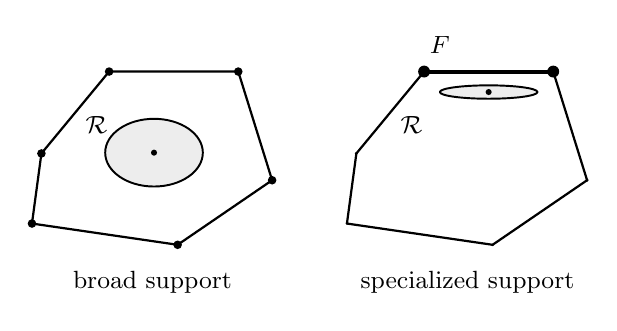
\begin{tikzpicture}[
  line cap=round,
  line join=round,
  every node/.style={font=\small},
  hull/.style={thick},
  local/.style={draw,fill=black!7,line width=0.7pt}
]

% ------------------------------------------------------------------
% Broad support
% ------------------------------------------------------------------
\begin{scope}[xshift=0cm]
  \coordinate (A1) at (0,0.45);
  \coordinate (A2) at (1.85,0.18);
  \coordinate (A3) at (3.05,1.00);
  \coordinate (A4) at (2.62,2.38);
  \coordinate (A5) at (0.98,2.38);
  \coordinate (A6) at (0.12,1.34);

  \draw[hull] (A1)--(A2)--(A3)--(A4)--(A5)--(A6)--cycle;

  \draw[local] (1.55,1.35) ellipse [x radius=0.62,y radius=0.43];
  \fill (1.55,1.35) circle (1.1pt);

  \foreach \P in {A1,A2,A3,A4,A5,A6}
    \fill (\P) circle (1.55pt);

  \node at (0.82,1.70) {$\mathcal R$};
  \node at (1.53,-0.30) {broad support};
\end{scope}

% ------------------------------------------------------------------
% Specialized support
% ------------------------------------------------------------------
\begin{scope}[xshift=4.00cm]
  \coordinate (B1) at (0,0.45);
  \coordinate (B2) at (1.85,0.18);
  \coordinate (B3) at (3.05,1.00);
  \coordinate (B4) at (2.62,2.38);
  \coordinate (B5) at (0.98,2.38);
  \coordinate (B6) at (0.12,1.34);

  \draw[hull] (B1)--(B2)--(B3)--(B4)--(B5)--(B6)--cycle;
  \draw[line width=1.4pt] (B5)--(B4);
  \node[anchor=south] at (1.18,2.48) {$F$};

  \draw[local] (1.80,2.12) ellipse [x radius=0.62,y radius=0.085];
  \fill (1.80,2.12) circle (1.1pt);

  \fill (B1) circle (0.50pt);
  \fill (B2) circle (0.50pt);
  \fill (B3) circle (0.60pt);
  \fill (B4) circle (2.15pt);
  \fill (B5) circle (2.15pt);
  \fill (B6) circle (0.60pt);

  \node at (0.82,1.70) {$\mathcal R$};
  \node at (1.53,-0.30) {specialized support};
\end{scope}

\end{tikzpicture}

\end{document}
